\chapter{Reconstrucción e identificación de objetos físicos}
% \addcontentsline{toc}{chapter}{Reconstrucción e identificación de objetos físicos}
\chaptermark{Reconstrucción e identificación de objetos físicos}

\tosolve{H: citar ICHEP? donde?}

En el presente capítulo se describe la reconstrucción e identificación de electrones y fotones ya que son los objetos físicos principales utilizados en los estudios de esta Tesis. La reconstrucción de fotones y electrones en ATLAS se basa en las deposiciones locales de energía halladas en el ECAL, y la distinción entre unos y otros se   realiza mediante la información de las trazas reconstruidas en el ID. A su vez se aplican una serie de criterios de identificación y aislamiento, que permiten discriminarlos de falsos candidatos, o de procesos secundarios que los producen.

\section{Reconstrucción de electrones y fotones}

La  reconstrucción de fotones y electrones en ATLAS se basa en un algoritmo de clusterización \cite{Lampl:1099735} que busca deposiciones locales de energía en el calorímetro dentro de una ventana rectangular en el espacio ($\eta$, $\phi$) de tamaño fijo (\textit{Sliding Window clusterization}, SW). La posición de la ventana se ajusta maximizando la energía transversa de todas las celdas contenidas. El tamaño óptimo de la ventana depende del tipo de partícula (más ancha para los electrones) a reconstruir y de la región del calorímetro (mas ancha en la región endcap). 

Aquellos \textit{clusters} electromagnéticos asociados con una traza reconstruida con $p_{T} > 0.5 \egev$, son clasificados como electrones. La definición para fotones es un poco más complicada ya que estos pueden convertir en un par $e^{+}e^{-}$ en el sector anterior al calorímetro. Los fotones convertidos están caracterizados por la presencia de al menos una traza asociada proveniente de un vértice reconstruido en el ID. La probabilidad de conversión varía entre un 40\% y un 80\% dependiendo de $\eta$, aunque solo aquellas que ocurren antes del TRT son eficientemente reconstruidas. 

Si no hay ninguna traza asociada a un dado \textit{cluster}, este es clasificado como un fotón no convertido. Aquellos \textit{clusters} asociados con trazas, que provienen de un vértice reconstruido en el ID, es clasificado como un fotón convertido. Además, para incrementar la eficiencia de reconstrucción de estos últimos, se consideran también aquellos casos donde solo una traza fue reconstruida, siempre que esta no posea ningún impacto en el B-Layer.

\section{Identificación de electrones y fotones}

La identificación de fotones se lleva a cabo mediante una serie de cortes rectangulares en un conjunto de variables que describen la forma y la estructura de las lluvias electromagnéticas según se propagan en el detector. Estas variables incluyen información de los calorímetros y, para el caso de fotones convertidos, del detector de trazas. Se definen dos conjuntos de cortes dependiendo de la rigurosidad de los mismos: \textit{loose} y \textit{tihgt}. Los cortes de cada conjunto han sido optimizados para asegurar una alta eficiencia de identificación de electrones/fotones aislados y de rechazo de fondo. 

Para la identificación de electrones se utiliza un algoritmo de identificación basado en el método de \textit{likelihood} (LH). El mismo consiste en una técnica de análisis multivariable que evalua simultáneamente distintas propiedades de los candidatos a la hora de realizar la selección. El LH utiliza las funciones de densidad de probabilidad (PDFs) de la señal y del fondo de las distintas variables que describen a la lluvia electromagnética. Basada en esas PDFs, se calcula una probabildiad total del objeto de ser señal o fondo. Adicionalmente se utilizan variables discriminantes que se basan en la cantidad de impactos en el detector de trazas. Se utilizan tres cortes de discriminación: \textit{loose}, \textit{medium} y \textit{tihgt}. Los mismos se definen de tal forma de que los objetos seleccionado por uno sean un subconjunto de los otros. Es decir, los seleccionados por \textit{medium} son sleccionados también por \textit{loose}, y los seleccionados por \textit{tihgt} son sleccionados también por \textit{medium}.


La definición de algunas variables que determinan los distintos cortes se detallan a continuación. La definición de los cortes se muestra en la Tabla \ref{lmttable}.


\begin{itemize}

	\item \textbf{Fuga hadrónica}

		Es la energía transversa depositada en el calorímetro hadrónico, normalizada a la energía transversa del cluster electromagnético.

		\begin{equation}
		R_{\text{had}_{(1)}}=\frac{E_{T}^{\text{had}}}{E_{T}}
		\end{equation}

		En la región de transición barrel-endcap del HCAL, se utiliza el depósito de energía en todo el calorímetro hadrónico para minimizar los efectos de la degradación de resolución ($R_{\text{had}}$). En el resto del detector, se mide sólo la energía hadrónica depositada en la primera capa del HCAL ($R_{\text{had}_{(1)}}$).

	\item  \textbf{Perfil lateral de energía en $\eta$ (2$^{\text{da}}$ capa del ECAL)}

		\begin{equation}
		R_{\eta}=\frac{E_{3\times 7}^{S2}}{E_{7\times 7}^{S2}}
		\end{equation}

 		donde $E_{i\times j}^{S2}$ es la suma de las celdas en la segunda capa del calorímetro electromagnético contenidas en una ventana $i\times j$ (en $\Delta \eta \times \Delta \phi$).

	\item  \textbf{Perfil lateral de energía en $\phi$ (2$^{\text{da}}$ capa del ECAL)}

		\begin{equation}
		R_{\phi}=\frac{E_{3\times 3}^{S2}}{E_{3\times 7}^{S2}}
		\end{equation}

 		donde $E_{i\times j}^{S2}$ es la suma de las celdas en la segunda capa del calorímetro electromagnético contenidas en una ventana $i\times j$ (en $\Delta \eta \times \Delta \phi$).

	\item  \textbf{RMS del perfil lateral de energía en $\eta$ (2$^{\text{da}}$ capa del ECAL)}


		\begin{equation}
		w_{\eta_{2}}=\sqrt{\frac{\sum E_{i}\eta_{i}^{2}}{\sum E_{i}}- \left(\frac{\sum E_{i}\eta_{i}}{\sum E_{i}}\right)^{2}}
		\end{equation}

		mide el ancho lateral de las lluvias electromagnéticas, donde $E_{i}$ es la energía de la i-ésima celda del calorímetro electromagnético contenida en una ventana de $3\times 5$ celdas en $\eta \times \phi$.

	\item  \textbf{Perfil lateral de energía en $\eta$ (1$^{\text{ra}}$ capa del ECAL)}

		\begin{equation}
		F_{\text{side}}=\frac{E(\pm 3)-E(\pm 1)}{E(\pm 1)}
		\end{equation}

		mide la contención lateral de la cascada electromagnética a lo largo de $\eta$. $E(\pm n)$ es la energía en las $\pm n$ celdas alrededor de aquella con la deposición máxima.

	\item  \textbf{RMS del perfil lateral de energía en $\eta$ (3 \textit{strips}, 1$^{\text{ra}}$ capa del ECAL)}

		\begin{equation}
		w_{s,3}=\sqrt{\frac{\sum E_{i}(i-i_{\text{max}})^{2}}{\sum E_{i}}}
		\end{equation}

		mide el ancho de la lluvia electromagnética a lo largo de $\eta$ en la primera capa del calorímetro electromagnético usando solo la banda con mayor deposición de energía ($i_{\text{max}}$) y sus vecinas inmediatas.

	\item  \textbf{RMS del perfil lateral de energía en $\eta$ (total, 1$^{\text{ra}}$ capa del ECAL)}

		$w_{s,\text{tot}}$ está definida de la misma forma que $w_{s,3}$, pero utiliza todas las bandas de la primera capa del calorímetro electromagnético en una ventana $\Delta\eta\times\Delta\phi = 0.0625 \times 0.2$, que corresponde aproximadamente a $20\times 2$ bandas en $\eta \times \phi$.

	\item  \textbf{Diferencia al segundo máximo}

		\begin{equation}
		\Delta E=[E_{2^{nd} \:\text{max}}^{S1} - E_{\text{min}}^{S1}]
		\end{equation}

		es la diferencia entre la energía de la banda con la segunda energía más grande $E_{2^{nd} \:\text{max}}^{S1}$ , y la mínima energía $E_{\text{min}}^{S1}$ entre la anterior y la celda con la máxima deposición. En caso de no haber segundo máximo se fija $\Delta E = 0$.

	\item  \textbf{Asimetría de los dos máximos locales en $\eta$}

		\begin{equation}
		\Delta E_{\text{ratio}}=\frac{E_{1^{st} \:\text{max}}^{S1} - E_{2^{nd} \:\text{max}}^{S1}}{E_{1^{st} \:\text{max}}^{S1} + E_{2^{nd} \:\text{max}}^{S1}}
		\end{equation}
 
 		mide la diferencia relativa entre las energías de las dos celdas con máxima deposición. En caso de no haber segundo máximo se fija $E_{\text{ratio}} = 1$.


\end{itemize}

\renewcommand{\arraystretch}{1.0}
\begin{table}	
\centering
\caption{Detalle de las diferentes variables usadas para la selección \textit{loose} (L) y \textit{tight} (T) de fotones y electrones. El $\checkmark$ indica cuándo la selección requiere de esa variable. \cite{ATLAS:2016iqc} \cite{Tripiana:1433788}}
 \makebox[0.5\textwidth][c]{
 \begin{tabular}{ r p{8cm} c | c c | c }

	\hline

	\multirow{2}{*}{Categoría} & \multirow{2}{*}{Descripción} & \multirow{2}{*}{Nombre} & \multicolumn{2}{ c |}{$\gamma$} & \multirow{2}{*}{$e$} \\

		&	&	& L & T &   \\

	\hline

	Aceptancia & $|\eta| < 2.37$, excluyendo $1.37 < |\eta| < 1.52$  & - & $\times$ & $\checkmark$ & $\times$  \\

	Fuga hadrónica & Cociente entre $E_{T}$ en la primera capa del calorímetro hadrónico y $E_{T}$ del \textit{cluster} electromagnético & $R_{\text{had}_{1}}$ & $\checkmark$ & $\checkmark$ & $\checkmark$ \\

		& Cociente entre $E_{T}$ en todo el calorímetro hadrónico y $E_{T}$ del \textit{cluster} electromagnético $(|\eta| \le 0.8$ y $|\eta| \ge 1.37)$ & $R_{\text{had}}$ & $\checkmark$ & $\checkmark$ & $\checkmark$  \\

	ECAL (3$^{ra}$ capa) & Fracción de energía en la tercer capa del ECAL & $f_{3}$ & $\times$ & $\times$ & $\checkmark$  \\
	

	ECAL (2$^{da}$ capa) & Ancho lateral de la lluvia en dirección de $\eta$ & $w_{\eta_{2}}$ & $\checkmark$ & $\checkmark$ & $\checkmark$ \\

		& Cociente entre la suma de las energías de las 3 $\times$ 7 celdas y la suma de 5 $\times$ 7 celdas, ambas en torno al centro del \textit{cluster} & $R_{\eta}$ & $\checkmark$ & $\checkmark$ & $\checkmark$ \\

		& Cociente entre la suma de las energías de las 3 $\times$ 3 celdas y la suma de 3 $\times$ 7 celdas, ambas en torno al centro del \textit{cluster} & $R_{\phi}$ & $\times$ & $\checkmark$ & $\checkmark$ \\

	ECAL (1$^{ra}$ capa) & Ancho lateral de la lluvia en 3 \textit{strips} alrededor del máximo & $w_{s,3}$ & $\times$ & $\checkmark$ & $\times$ \\

		& Ancho lateral total de la lluvia & $w_{s,\text{tot}}$ & $\times$ & $\checkmark$ & $\checkmark$ \\

		& Fracción de energía fuera de las 3 \textit{strips} centrales pero dentro de las 7 & $F_{\text{side}}$ & $\times$ & $\checkmark$ & $\times$ \\

		& Diferencia entre la energía de la \textit{strip} con el segundo mayor depósito y la menor energía entre los dos primeros máximos locales & $\Delta E$ & $\times$ & $\checkmark$ & $\times$ \\

		& Asimetría entre el primer y segundo máximo & $E_{\text{ratio}}$ & $\times$ & $\checkmark$ & $\checkmark$  \\

		& Fracción de energía en la primera capa del ECAL & $f_{1}$ & $\times$ & $\times$ & $\checkmark$  \\

	ID & Parámetro de impacto transverso& $d_{0}$ & $\times$ & $\times$ & $\checkmark$ \\

		& Momento perdido en la traza entre el primer punto de detección y el último, dividido el momento total original & $\Delta p/p$ & $\times$ & $\times$ & $\checkmark$  \\

	TRT & Probabilidad \textit{likelihood} basa en la radiación de transición en el TRT & eProbabilityHT & $\times$ & $\times$ & $\checkmark$  \\

	ECAL+ID & $\Delta\eta$ entre la traza extrapolada al calorímetro y el \textit{cluster} en la primer capa& $\Delta\eta_{1}$ & $\times$ & $\times$ & $\checkmark$ \\

	\hline

\end{tabular}}
\label{lmttable}
\end{table}
\renewcommand{\arraystretch}{1}

Por último un algoritmo adicional es aplicado para resolver ambigüedades residuales en para candidatos de fotones que son también reconstruidos como electrones. Diferentes estrategias son utilizadas dependiendo del estado de conversión de los fotones según es explica en la Referencia \cite{ambiguity}.


\section{Criterios de aislamiento}

Luego de realizar la identificación, es necesario distinguir entre electrones y fotones directos (aquellos producidos en la colisión) o de los no directos producidos de decaimientos de hadrones ($\pi^{0}$, $\eta$, etc.) dentro de jets \tosolve{H: o mal reconstruidos?}.

Los fotones o electrones provenientes del punto de interacción, o los electrones provenientes de $Z\rightarrow ee$, poseen baja actividad hadrónica en su vecindad, mientras que en los no directos se espera que haya un gran actividad provenientes de los objetos que acompañan al jet. Para realizar esta identificación se utiliza un criterio de aislamiento que se basa en medidas calorimétricas o en las trazas reconstruidas en el entorno del objeto.

El aislamiento de trazas se define a partir de considerar un cono de radio $R=\sqrt{\Delta\eta^{2}+\Delta\phi^{2}}$ centrado en el baricentro del \textit{cluster} electromagnético asociado al objeto. A todas las trazas dentro de este cono se le pueden aplicar ciertos cortes, como $p_{T}>1 \egev$, impactos en el SCT, etc. Además, se requiere que aquellas trazas en un cono interno con $R=0.1$, no provengan de un vértice de conversión, a fin de remover los fotones convertidos. El aislamiento de trazas ha mostrado ser altamente eficiente tanto para retener señal como para rechazar falsos candidatos del fondo, aún luego de la selección descripta en la sección anterior. Aun así, el criterio más utilizado es el aislamiento calorimétrico.

El aislamiento calorimétrico, $E_{T}^{\text{iso}}$, se calculada a partir de las celdas en ambos calorímetros (ECAL y HCAL). Nuevamente se define un cono con un cierto radio $R$ centrado en el baricentro del \textit{cluster} del objeto, y la suma de la energías de todas las celdas contenidas en ese cono se denomina $E_{T}^{\text{iso}}$. 

A fin de remover la contribución energética de la lluvia electromagnética desarrollada por el propio objeto al cono de aislamiento, el núcleo central de $N_{\eta}\times N_{\phi} = 5 \times 7$ celdas en el segundo compartimiento del ECAL, es ignorado en la suma, como se esquematiza en la Figura \ref{isolation}. Se considera que dentro de esta región ignorada, se concentra el 95\% de la energía de la lluvia electromagnética, por lo que solo el 5\% de la energía del objeto contribuye a esta región. Por otro lado, todas las celdas contenidas dentro del cono en el HCAL son consideradas para la suma, ya que se espera que el ECAL contenga toda lluvia electromagnética desencadenada por el objeto inicial. 

Para fotones, el valor típico de $R$ es $0.4$, y los cortes de aislamiento son \tosolve{No entiendo lo que dice} $E_{T}^{\text{iso}}<2.45 \egev + 0.022 \times p_{T}$. En cambio en los electrones pasan por un criterio denominando \textit{Gradient Loose}, en el cual el valor de $R$ depende del $p_{T}$ de los mismos. En este caso para el aislamiento calorimétrico $R=0.2$ y para el aislamiento de trazas $R=10\egev/p_{T}$

\begin{figure}
\centering
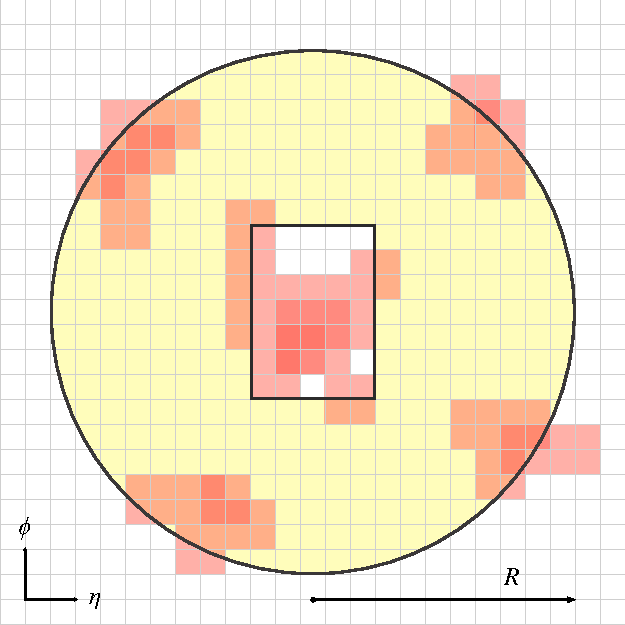
\includegraphics[width=0.50\textwidth]{iso.pdf}
\caption{Esquema ilustrando el cálculo de la energía de aislamiento del fotón. La \textit{grid} representa la granularidad de las celdas del calorímetro electromagnético. El cono de color amarillo de radio $R$ rodea al candidato. La energía del candidato a fotón o electrón está mayormente contenida en el rectángulo central de $5 \times 7$ en $\Delta\eta \times \Delta\phi$.}
\label{isolation}
\end{figure}

\section{Energía faltante}

Una variable de suma importancia en la búsqueda de partículas supersimétricas, es la energía transversa faltante ($\met$). Como se mencionó anteriormente, el momento transverso se debe conservar en todo el proceso, y cualquier desequilibrio en el mismo se lo asocia a $\met$. Puede indicar la presencia de partículas indetectables como neutrinos o nuevas partículas estables, o que interactúan débilmente con la materia.

El momento transverso faltante ($p_{T}^{\text{miss}}$) se define como el valor negativo de la suma del momento transverso de todas las partículas detectadas, y su magnitud es lo que se denomina energía transversa faltante. Esta es calculada con un algoritmo basado en objetos \cite{Khoo:2012749}. El algoritmo utiliza los objetos físicos construidos y calibrados descriptos en las secciones anteriores. Los depósitos de energía en el calorímetro (topo-clusters) son asociados a los objetos de alto $p_{T}$ en el siguiente orden: electrones, fotones, jets y muones. Los depósitos que no están asociados a ningún objeto son incluidos en el término \textit{soft}. El momento transverso es calculado entonces como:

\begin{equation}
p_{T}^{\text{miss}}=\left(p_{T}^{\text{miss}}\right)^{e} + \left(p_{T}^{\text{miss}}\right)^{\gamma} + \left(p_{T}^{\text{miss}}\right)^{\text{jet}} +\left(p_{T}^{\text{miss}}\right)^{\mu} + \left(p_{T}^{\text{miss}}\right)^{\text{soft}}
\end{equation}
%
donde cada término es calculado como el negativo de la suma de los objetos reconstruidos y calibrados, más el término \textit{soft}. La contribución de los taus, se incluye en el término de jets o en el \textit{soft}, debido a que los mismos decaen hadrónicamente. Finalmente la energía transversa faltante se define como:

\begin{equation}
\met=|p_{T}^{\text{miss}}|
\end{equation}

